\documentclass{article}
\newsavebox{\oldepsilon}
\savebox{\oldepsilon}{\ensuremath{\epsilon}}
\usepackage[minionint,mathlf,textlf]{MinionPro} % To gussy up a bit
\renewcommand*{\epsilon}{\usebox{\oldepsilon}}
\usepackage[margin=1in]{geometry}
\usepackage{graphicx} % For .eps inclusion
%\usepackage{indentfirst} % Controls indentation
\usepackage[compact]{titlesec} % For regulating spacing before section titles
\usepackage{adjustbox} % For vertically-aligned side-by-side minipages
\usepackage{array, amsmath,  mhchem}
\usepackage[hidelinks]{hyperref}
\usepackage{courier, subcaption}
\usepackage{multirow, enumerate}
\usepackage[autolinebreaks,framed,numbered]{mcode}

\usepackage{float}
\restylefloat{table}

\pagenumbering{gobble} 
\setlength\parindent{0 cm}
\renewcommand{\arraystretch}{1.2}
\begin{document}
\large

MCB 135 Problem Set 5 \hfill Due Monday, March 9, 2015 at 2:30 PM

\section*{Problem 1: Working with proteomics data (50 points)}

In this problem, you will explore the protein-protein interaction network recently described by \linebreak \href{http://www.cell.com/abstract/S0092-8674\%2814\%2901422-6}{Rolland et al. (2014)}. The interactions are provided in tab-delimited format on the course \linebreak website (\mcode{rolland.tsv}). Each line describes one interaction: the two columns give the \href{http://www.ncbi.nlm.nih.gov/gene}{NCBI \linebreak Entrez gene identification numbers} for the two proteins participating in the interaction.

\begin{enumerate}[a)]
\setlength{\itemsep}{0pt}
\item Determine the number of interactions in which each protein participates. (The MATLAB \linebreak functions \mcode{unique()} and \mcode{histcounts()} may be useful.) Find the average number of interactions per protein, $\mu$.
\item Plot the distribution of interactions per protein -- i.e., the probability that a randomly-chosen protein participates in $x$ interactions -- on log-log axes.
\end{enumerate}
Under the hypothesis that all possible edges in a network occur with equal probability, the number of edges per node is expected to follow a Poisson distribution. 
\begin{enumerate}[a)]
\setlength{\itemsep}{0pt}
\setcounter{enumi}{2}
\item Plot a Poisson distribution with parameter $\mu$ on the same axes as the true distribution of interaction counts. In MATLAB, this can be done with the function \mcode{poisspdf()}.
\end{enumerate}
An alternative ``preferential attachment" model holds that new edges are connected preferentially to nodes that already have many edges. In the resulting ``scale-free" network, the distribution of edges per node follows a power law.
\begin{enumerate}[a)]
\setlength{\itemsep}{0pt}
\setcounter{enumi}{3}
\item  Fit a power law to the data and plot it on the same axes as in parts (b) and (c). In MATLAB, this can be done with the function \mcode{fit(x,y,'power1')}.
\item Which distribution -- Poisson or power law -- is a better fit to the Rolland et al. data? Explain why this distribution be expected in light of how protein-protein interactions evolve.
\item How many self-interactions are reported in this data set? How many self-interactions would you have expected given the number of proteins and the total number of interactions? (You may assume that all edges are equally likely, even if that assumption does not match your results from part e.)
\item Provide a biological justification for any discrepancy between the two values found in part f.
\end{enumerate}

\section*{Problem 2: Autorepression with a time delay (50 points)}


In lecture, we studied an autoregulating transcriptional repressor to find its protein abundance $p(t)$ as a function of an input, $x(t)$, that drives the gene's transcription:

\begin{center}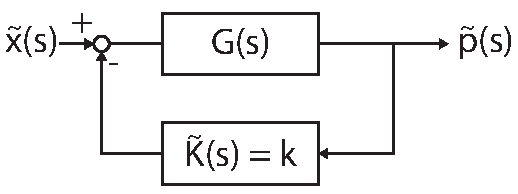
\includegraphics[width=0.4 \textwidth]{autorepression.pdf}\end{center}

We now consider a modified version of this model in which there is a delay $\tau$ between mRNA production and translation\footnote{In eukaryotes, transcriptional elongation, mRNA processing, and nuclear export introduce delays (usually on the order of minutes) between the initiation of transcription and the initiation of translation.}. This delay is reflected in the modified rate equations:
\begin{eqnarray}
\begin{aligned}
\frac{d m}{dt} & = & c_m a(t) - \gamma_m m(t)\\
\frac{d p}{d t} & = & c_p m(t-\tau) - \gamma_p p(t) \label{eqn:rateequations}
\end{aligned}
\end{eqnarray}

\noindent where $a(t)$, the mRNA's net expression level, is $x(t)-k p(t)$ (the activating input minus the strength of the negative autoregulation).

\begin{enumerate}[a)]
\setlength{\itemsep}{0pt}
\item Show using the definition of the Laplace transform that for a function $f(t)$ which is non-zero only for positive $t$,
\[ \mathcal{L}\left[f(t-\tau)\right] = e^{-s\tau} \mathcal{L}\left[f(t)\right] = e^{-s\tau} \tilde{f}(s)\]
\item Transform rate equations (\ref{eqn:rateequations}) and simplify to find an expression for the forward transfer \linebreak  function $G(s) =\tilde{p}(s)/\tilde{a}(s)$. Assume that $m(0)=p(0)=0$.
\item Find an expression for the closed loop transfer function $\tilde{p}(s)/\tilde{x}(s)$ in terms of $k$ and $G(s)$.
\end{enumerate}
The autorepression system is unstable if any poles of the closed loop transfer function have a positive real part.
\begin{enumerate}[a)]
\setlength{\itemsep}{0pt}
\setcounter{enumi}{3}
\item Show that the only poles of the closed loop transfer function which could have a positive real part are the roots of $1 + kG(s)$.
\end{enumerate}
The result in part (d) implies that the system will be unstable if any roots of $1 + kG(s)$ have a positive real part. The Nyquist stability criterion can be used to determine whether any such roots exist, but in order to apply it, we must first know the number of poles of $1 + kG(s)$ with a positive real part.
\begin{enumerate}[a)]
\setlength{\itemsep}{0pt}
\setcounter{enumi}{4}
\item Demonstrate that the number of poles of $1 + kG(s)$ with positive real part is zero.
\end{enumerate}
The absence of poles with positive real part implies that the number of zeros of $1 + kG(s)$ with positive real part is equal to the number of times that the Nyquist plot of $1 + kG(s)$ encloses the origin clockwise. Equivalently, the system is stable if the Nyquist plot of $G(s)$ does not enclose the point $-1/k$.

\begin{enumerate}[a)]
\setlength{\itemsep}{0pt}
\setcounter{enumi}{5}
\item Show that $G(s) \to 0$ as $|s| \to \infty$. [The Nyquist plot is therefore well approximated by $G(s=i\omega)$ for $\omega \in (-n, n)$ with sufficiently large $n$: we can ignore other points on the Nyquist contour.]
\item Use MATLAB to plot $G(i\omega)$ on the complex plane for $\omega \in (-100, 100)$. Use $c_i=\gamma_i=1$ and two values of $\tau$: 0 and 1.
\item Show using your $\tau=1$ Nyquist plot that there exists a threshold gain $k^*$ above which the system is unstable. (Though you will not show it explicitly, this is true for all $\tau,c_i, \gamma_i>0$.) Confirm from the $\tau=0$ Nyquist plot that the system is stable for all $k$ when there is no time delay.
\item Approximately what value of the repressor's gain $k$ would be ideal when $\tau=c_i=\gamma_i=1$? (That is, what value of $k$ minimizes the deviation of $p(t)$ from zero in this case?)
\item The repressor's gain $k$ can be adjusted through mutation and natural selection. Describe two types of mutations that could alter the value of $k$.
\end{enumerate}

\end{document}